\documentclass[12pt,a4paper,oneside]{report}

\usepackage{amsmath}
\usepackage{amsfonts}
\usepackage{cite}
\usepackage{graphicx}
\usepackage{epstopdf}
\usepackage[bookmarks]{hyperref}
\usepackage{verbatim}
\usepackage[nottoc,numbib]{tocbibind}
\usepackage{datatool}
\usepackage[acronym,nomain,toc,nonumberlist]{glossaries}
\usepackage[numbered,framed,final]{matlab-prettifier}
\usepackage{setspace}
\usepackage[lofdepth,lotdepth]{subfig}


\onehalfspacing

% Generate the glossary

% fix the system to capitalize all first letters, not just the first
\makeatletter
\let\oldmakefirstuc\makefirstuc
\renewcommand*{\makefirstuc}[1]{%
  \def\gls@add@space{}%
  \mfu@capitalisewords#1 \@nil\mfu@endcap
}
\def\mfu@capitalisewords#1 #2\mfu@endcap{%
  \def\mfu@cap@first{#1}%
  \def\mfu@cap@second{#2}%
  \gls@add@space
  \oldmakefirstuc{#1}%
  \def\gls@add@space{ }%
  \ifx\mfu@cap@second\@nnil
    \let\next@mfu@cap\mfu@noop
  \else
    \let\next@mfu@cap\mfu@capitalisewords
  \fi
  \next@mfu@cap#2\mfu@endcap
}
\makeatother

% Glossary Term definitions
\newacronym{puf}{PUF}{physically unclonable function}
\newacronym{crp}{CRP}{challenge-response pair}
\newacronym{cra}{CRA}{challenge-response authentication}
\newacronym{pin}{PIN}{personal identification number}
\newacronym{mitm}{MitM}{man-in-the-middle}
\newacronym{sram}{SRAM}{static random-access memory}
\newacronym{mosfet}{MOSFET}{metal-oxide semiconductor field-effect transistor}
\newacronym{ip}{IP}{intellectual property}
\newacronym{fpga}{FPGA}{field-programmable gate array}
\newacronym{rf}{RF}{radio frequency}
\newacronym{rfid}{RFID}{radio-frequency identification}
\newacronym{ecc}{ECC}{error-correcting code}
\newacronym{vhdl}{VHDL}{VHSIC hardware description language}
\newacronym{vhsic}{VHSIC}{very high speed integrated circuit}
\newacronym{asic}{ASIC}{application-specific integrated circuit}
\newacronym{rng}{RNG}{random number generator}
\newacronym{trng}{TRNG}{true random number generator}
\newacronym{prng}{PRNG}{pseudo-random number generator}
\newacronym{sha}{SHA}{secure hash algorithm}
\newacronym{nsa}{NSA}{national Security Agency}
\newacronym{sha2}{SHA-2}{secure hash algorithm, version 2}
\newacronym{xor}{XOR}{exclusive disjunction}
\newacronym{lan}{LAN}{local area network}
\newacronym{aes}{AES}{advanced encryption standard}
\newacronym{wep}{WEP}{Wired Equivalent Privacy}
\newacronym{wpa}{WPA}{wi-fi protected access}
\newacronym{wpa2}{WPA2}{wi-fi protected access version two}
\newacronym{wps}{WPS}{wi-fi protected setup}
\newacronym{slip}{SLIP}{serial line Internet protocol}
\newacronym{ppp}{PPP}{point to point protocol}
\newacronym{pots}{pots}{plain old telephone system}
\newacronym{pppoe}{PPPoE}{PPP over ethernet}
\newacronym{uart}{UART}{universal asynchronous receiver/transmitter}
\newacronym{pae}{PAE}{port access entity}
\newacronym{eap}{EAP}{extensible authentication protocol}
\newacronym{eap-otp}{OTP}{EAP one time password/pad}
\newacronym{gsm}{GSM}{global system for mobile communications}
\newacronym{umts}{UMTS}{universal mobile telecommunications system}
\newacronym{eapol}{EAPoL}{EAP over LAN}
\newacronym{crc}{CRC}{cyclic redundancy check}
\newacronym{macsec}{MACSec}{MAC Security}
\newacronym{icv}{ICV}{MACSec message authentication code}
\newacronym{mac}{MAC}{medium access control}
\newacronym{mac2}{MAC}{message authentication code}
\newacronym{tls}{TLS}{transport layer security}
\newacronym{ssl}{SSL}{secure socket layer}
\newacronym{https}{HTTPS}{hypertext transfer protocol secure}
\newacronym{otp}{OTP}{one time pad}
\newacronym{uba}{UBA}{upper byte access}
\newacronym{lba}{LBA}{lower byte access}
\newacronym{rtl}{RTL}{register transfer level}
\newacronym{ascii}{ASCII}{american standard code for information interchange}
\newacronym{msb}{MSB}{most significant bit}
\newacronym{lsb}{LSB}{least significant bit}
\newacronym{piso}{PISO}{parallel in, serial out}
\newacronym{sipo}{SIPO}{serial in, parallel out}
\newacronym{iana}{IANA}{internet assigned numbers authority}
\newacronym{radius}{RADIUS}{remote authentication dial in user service}
\newacronym{dos}{DoS}{denial of service}
\newacronym{fcs}{FCS}{frame check sequence}
\newacronym{nak}{NAK}{negative-acknowledgment}
\newacronym{lfsr}{LFSR}{linear feedback shift register}
\newacronym{rfc}{RFC}{request for comments}

\makeglossaries




% Run texcount on tex-file and write results to a sum-file
\immediate\write18{texcount -sum -1 -inc \jobname.tex -out=\jobname.sum}
% Define macro \wordcount for including the counts
\newcommand\wordcount{\input{\jobname.sum}}

% Macro for quick ways to enter common text
\newcommand{\matlab}{MATLAB\textsuperscript{\copyright}\ }
\newcommand{\inlinecode}{\texttt}
\newcommand{\HRule}{\rule{\linewidth}{0.5mm}}

\title{Physically Unclonable Functions for Networked Device Authentication}
\date{September, 2014}
\author{Michael Walker}

\begin{document}

% Front Matter
\pagenumbering{roman}
\input{meta/title}
% Declaration


\chapter*{Declaration} % Declaration section text

I declare that this dissertation represents my own work and that I have correctly acknowledged the work of others. This dissertation is in accordance with University and School guidance on good academic conduct (University guidance is available at \url{www.ncl.ac.uk/right-cite}).

\vspace{1.5cm}

% Space for signature
\rule{0.7 \linewidth}{1pt}\\
\vspace{0.25cm}
\indent{Michael Walker, \today}

\cleardoublepage
% Summary

\chapter*{Summary} % Summary name

%-------------------------------------------------------------------------------
Physically Unclonable Functions are a relatively recent area of active research which can be seen as analogous to hardware fingerprints that potentially offer a way to provide low-cost, automated, trustworthy authentication of embedded systems.
As the infrastructure of networked devices grows in our homes and workplaces so too will the need to protect ourselves from `Hardware Trojans' and other threats.
In reviewing the state-of-the-art of `PUF's' and their potential incorporation into modern ciphers as cryptographic primitives using fuzzy extractors, the general significance and worth of an investigation into the implementation of practical Ethernet message authentication codes using Static RAM PUFs and Fuzzy Extractors as the core components is to be shown.		
\cleardoublepage
% Table of Contents - List of Tables/Figures/Listings and Acronyms

%-------------------------------------------------------------------------------
\setcounter{tocdepth}{2} % Depth of sections to include in the table of contents - currently up to subsections

\setcounter{secnumdepth}{3} % Depth of sections to number in the text itself - currently up to subsubsections

\tableofcontents

\clearpage

\listoffigures

\listoftables

%Print the glossary
\glsaddall
\setglossarystyle{altlist}
\printglossary
\clearpage


% Main Content
\pagenumbering{arabic}
% Chapter 1

\chapter{Introduction} % Chapter title

% For referencing the chapter elsewhere, use \autoref{ch:introduction} 
\label{ch:introduction} 

%-------------------------------------------------------------------------------

\Glspl{puf} are a relatively recent concept under much research.
By harnessing physical properties that are hard to simulate or copy, yet are
easy to sample from as a data stream source of for cryptographic key information,
an identification and authentication package can be constructed for any device
that contains or incorporates that physical property.
This is analogous to a biometric such as a fingerprint or iris, but one which
can be found in embedded electronic devices rather than human biology.

In this dissertation I will discuss my findings into the implementation of
a \gls{puf} system that would be of practical use if incorporated into a small
electronic embedded networked device for providing the means to authenticate that
device without requiring passwords or any other type of user intervention.
A naive setup for this would involve the extraction of data from a physical device
with the properties of a \gls{puf} in response to a challenge specifiying the
parameters used for extraction, all data sent in plaintext via a standard network protocol

This first step provides a simply \gls{crp} by which the device can provide
identity information, but as has been found in the course of the project,
this is not enough for a complete authentication solution for two reasons.
Firstly both the  challenge and the reponse are in plaintext and thus
completely open to an
adversary's use of attacks such as the' replay attack or the \gls{mitm} attack,
hence any practical system requires some use of modern cryptographic methods to
secure the data.
Secondly the nature of \glspl{puf} means they provide their
data somewhat unrealiably, this must be allowed for and mitigated.
The concept of fuzzy extraction shall therefore be introduced and explored as
a means to provide both of these necessary additions to the 
\gls{puf}-based authentication system by utilising the concepts of \glspl{ecc} and
cryptographic hashes.

In this scenario it is necessary that the device with the PUF authenticates
itself over a network to some central authenticator which issues the challenges 
to the device to prove its identity.
The networked device must then respond to the challenge correctly otherwise all
or part of the networking medium that the device requires is in some way
withheld by the authenticator.
By this means network security can be achieved without any human intervention.
This would surely be a important and neccesary
step in facilitating the likely future integration of innumerable inexpensive
embeddded systems into wireless home and office networks.
This is because, without burdening the user with any increased installation 
inconvience adaquate security provision can be provided.
The use of \glspl{puf} in this provision by the estabilshment of a network
security protocol was also investigated.

In the next chapter (chapter 2) I will report my background research into the
subjects of \glspl{puf} and the use of \gls{sram} as a \gls{puf} source. Then
the research on fuzzy extraction with focus on the usage of a class of \gls{ecc}
called BCH codes and a family of cryptographic hash functions called SHA-2. Finally
research into techniques to add \gls{puf}-based security provision into the
Ethernet protocol will be discussed.

In the third chapter this initial research is built upon with an explanation of
the design of systems and simulations that were built to analyse and experiment
with the concepts gleaned from the intital research. These designs broadly fit
into three areas of design effort.
\begin{itemize}
\item An implementation of a RS-232 based \gls{crp} system for data extraction from a
physical SRAM device.
\item The simulation of a complete fuzzy extractor system in \matlab.
\item The design of a modified Ethernet protocol for \gls{puf} authentication.
\end{itemize}

In the forth chapter the results of the practical implementations of the designs
are presented, followed in the fifth chapter by a discussion of the implications
of this study.





% Chapter 2

\chapter{Background Research} % Chapter title

\label{ch:background} % For referencing the chapter elsewhere, use \autoref{ch:background}

%TC:ignore
%This is the Background chapter, it should be approximately 4,000 Words in total.
%SRAM-PUF section should be approximately 1,500 words longs
%Fuzzy Extractor section should be approximately 1,500 words long.
%Forward error correction subsection should make up approximately 500 words.
%Cryptographic Hashing subsection should be about 500 words long.
%Networking section should be 1000 words in length.
%TC:endignore
%-------------------------------------------------------------------------------

The intention of this project is to investigate and implement in full - or in
part - a prototypical networked device that can be authenticated using a \gls{puf}.
As explained in the introduction, there are three areas under investigation.
In this chahpter are the findings from preliminary research undertaken for each
of the three areas. This is the foundation which supported the eventual system
design that will be discussed in the next chapter.

\section{Identity and Authentication}

Verificaton of identity is fundamental to this project, and so related concepts
and foundations should be explored. Firstly, it should be noted that
authentication is a different concept to authorization and accounting, although
the three together (AAA-security) are often considered as a whole, the focus in
this project is Authentication only.

\subsection{Challenge-Response}

In this project, \gls{cra} is foundation for authentication of device identity.
\Glspl{cra} isa commonly used concept in the authentication of devices on a
network. The concept is that the device to be authorized (hereby known as the
\emph{Supplicant}) is challenged by the device that controls access to the
network (hereby known as the \emph{Authenticator}). For each device to be identified
correctly, there must be at least one \gls{crp} associated with
each device and the supplicant must respond
with its correct response, otherwise access to the network is denied.

In the simplest case this could be as simple as a basic password check with a
unique password associated to each device/user. Thus, mutual authentication by a
shared secret is obtained.
However, if an attacker
can eavesdrop the communications channel, they can also see the password sent and
use a replay attack to gain access by spoofing the response of the original
supplicant. To make the system more secure, many \glspl{crp} can
be generated, thereby requiring an attacker to record all possible pairs to be
guaranteed access to the system. The probability of one-time access is
inversely proportional to the number of pairs, such that with sufficient pairs
the reply attack can be made statistically impossible.

There is one important complication; if a response can be
partially guessed solely through analysis of patterns in the ciphertext a
challenge generates (called information deduction) this weakens the system.
Therefore correlation of the challenge to the response should
be as near to the Shannon entropy limit as possible.

\subsection{Authentication Factors and Inherited Identity}

In network communications within a shared medium, the identities of the communicating devices
must be explicitly made so that they can be read by the intended recipient.
However, without security procedures in place, it is very simple and entirely
possible for any device
to claim the identity of another since there is no way to verify its provenance.
Thus, in mature networks some form of authentication protocol is introduced.
Authentication is generally performed using authentication factors, these can be stated
succinctly as one of three types;

\begin{itemize}
\item Knowledge - what you \emph{know}.
\item Ownership - what you \emph{have}.
\item Inheritance - what you \emph{are}.
\end{itemize}

In most cases of network authentication the first two factors are used, sometimes in combination.
In the case of knowledge factors examples include passwords and \glspl{pin}. In the case of
ownership factors, examples include \gls{rfid} tags and smart-cards.
These are extensively used for
current \gls{lan} authentication systems, for example the old \gls{wep} security scheme for the
IEEE 802.11 standard (branded as `Wi-Fi') required a password 10 to 26 Hexadecimal digits to
be physically entered by hand. In fact, secret keys of this type form an
integral part of hardware cryptographic primitives in conventional methods of authentication.
These necessarily rely on the digital storage of secret keys in non-volatile memory,
which has proven vulnerable to reverse engineering and side channel attacks.

Although less common, due to its more physical nature, Ownership factors include the `VideoGuard'
viewing cards that must be inserted into a set-top-box in order to authenticate the device over
a \gls{ppp} connection through the \gls{pots} to access encrypted digital
satellite or cable television channels. Ultimately these systems also rely on
the digital storage of keys, however, they are stored
within the smart-card and not the device itself. If an exploit is found, new protocols with changed
smart-card designs can be implemented and replacements distributed to upgrade the security of the system.
This incurs a significant additional expense, but allows for far greater longer-term security.

In contrast, inheritance factors are very uncommon in authentication of network devices, and
more usually are used to authenticate users themselves in the form of biometrics such as fingerprints,
iris-scans and facial recognition.
The advantages of inheritance factors over traditional methods for networked devices should
be clear;
\begin{itemize}
\item Increased Convenience - Automates process, nothing to be forgotten or misplaced by the users
\item Increased Security - No passwords on scraps of paper, or smart-cards in wallets to be stolen,
  and nothing is easily guessable or easily duplicated.
\item Increased Accountability - Auditing and post-factum reporting are stronger, as identities are harder to forge or alter.
\end{itemize}

While humans and other biological systems have biometrics that can be used in this way, it is
less obvious that electronic hardware systems can make use of Inheritance factors.
\Glspl{puf} are an enabling technology that can allow this.
By making use of them we can transfer much of
the beneficial techniques found in the application of
biometrics to user-centric security systems to
the topic of of device-centric authentication.

\section{PUFs \& SRAM}

The first thing required for a \gls{puf} based authentication system is a \gls{puf}.
Introduced in 2002\cite{pappu2002puf},
\glspl{puf} can be built from a wide variety of technologies.
Some have
electronic construction, some not, and new designs seem to appear every year.
Of those \glspl{puf} that are created from electronic circuits, there are some
that can use off-the-shelf components and some that must be custom made in
silicon. There are some that are delay based\cite{maiti2010large} and some that
are based on memory state meta-stability.
\gls{sram} \glspl{puf} that use the meta-stability of the standard six transistor
\gls{sram} cell (see \autoref{fig:sram}) were initially proposed by
Guadardo\cite{guajardo2009puf}, and are the focus of this project.

\begin{figure}
  \centering
  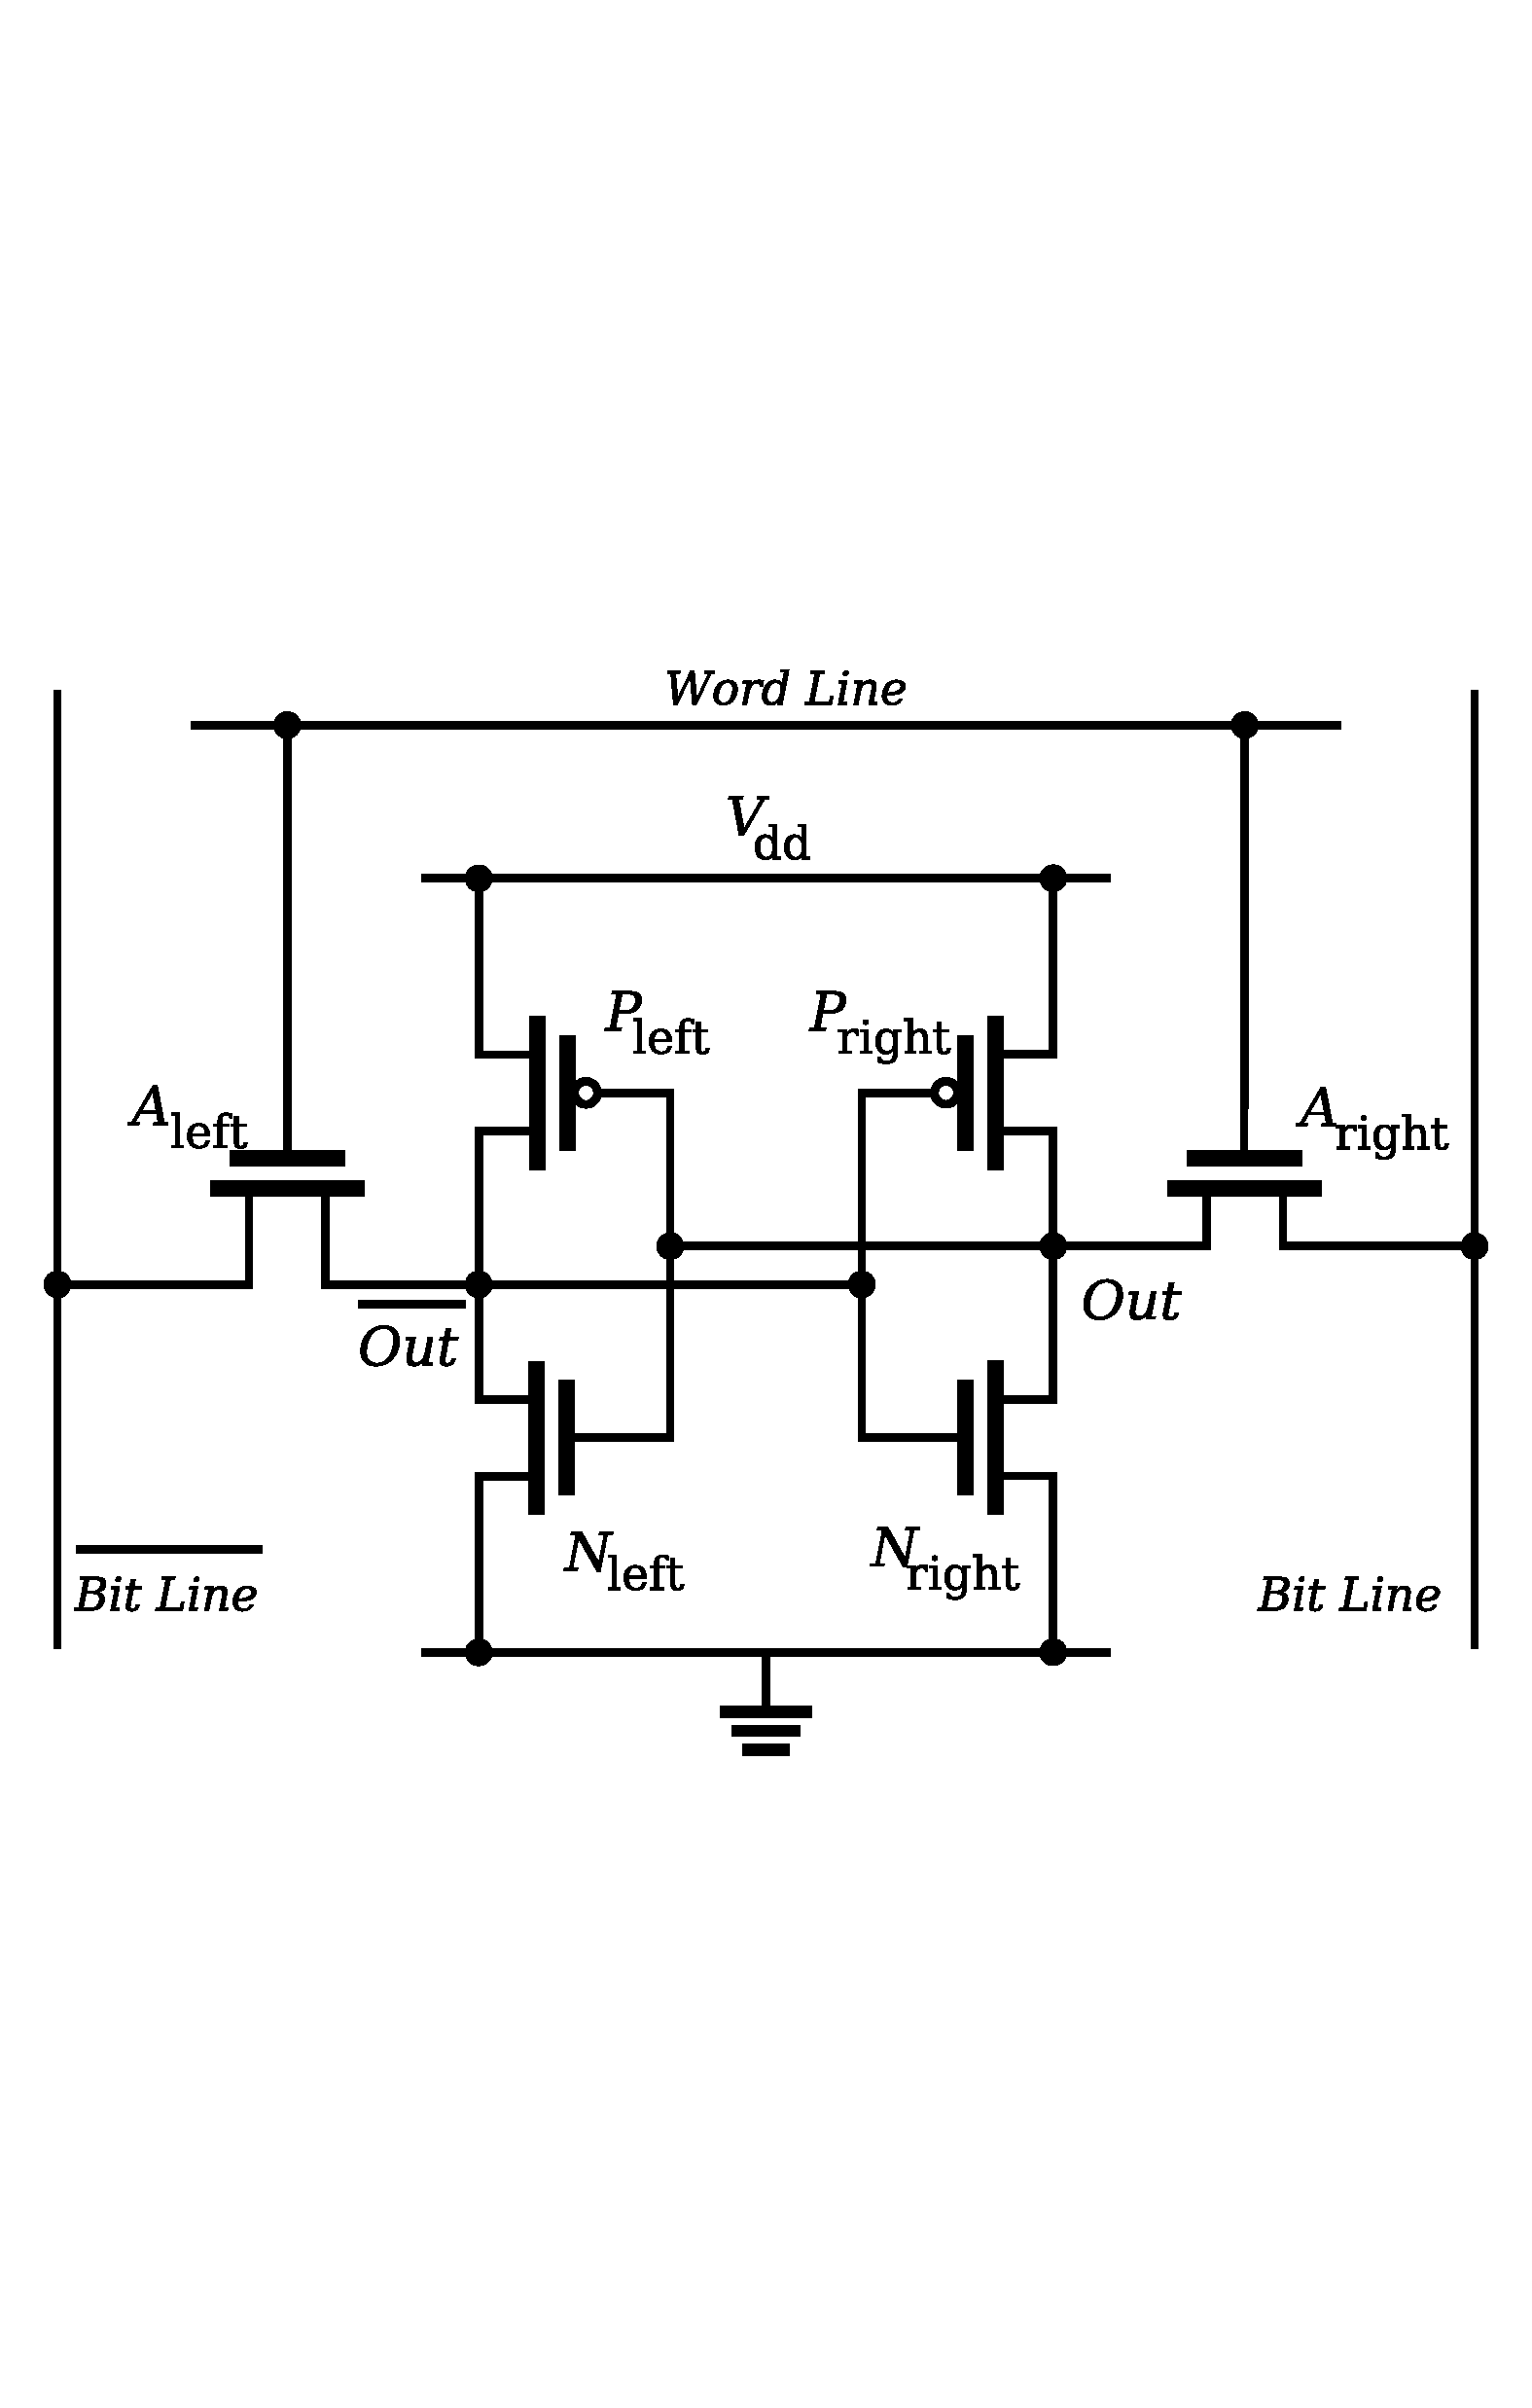
\includegraphics[scale=0.4, trim=0 300 0 300, clip]{images/sram}
  \caption{Six transistor SRAM diagram}
  \label{fig:sram}
\end{figure}

An \gls{sram} cell is conventionally constructed from \glspl{mosfet} in the
ubiquitous, modern photo-lithography process.
Any imperfections in the fabrication of the cell\footnote{such as subtle
variances in the transistors size, tiny changes in performance
characteristics due to silicon impurities, or any other of minute variance in
any of a thousand manufacturing steps} will result in a cell that is
predisposed to initialise to a particular binary value.
This meta-stability is a central underlying principal for the \glspl{sram}
functionality. Much research has been made into how the physical properties
of SRAM relate to it's use in
PUFS\cite{vandenberg2013analysis, maiti2013compare,maes201265nm}.
This project, however, will focus simply on the use of the unclonable entropy provided
by a PUF once it is created. It should be noted that authentication is only one
possible application of \glspl{puf}, and they have potential application in a wide
array of future technology including \glspl{trng}.

To construct an \gls{sram} based \gls{puf} either the \gls{sram} must be
incorporated into the design of an \gls{ip} core on the \gls{asic} itself,
or it could be accessed from outside.
In a practical \gls{puf} core of an embedded device, the former may be easier
to implement, but the latter would take less space.
In the case of this project, where a physical \gls{ip} core will not be
implemented, the functionality is intended to reside in an \gls{fpga}.
The acquisition of a separate \gls{sram} device is required as a basic
\glspl{fpga} chip itself is unlikely to have the memory quantity required.
For example, in this project a Cyclone II 2C20 FPGA device is used which contains
32 M4K RAM blocks yielding a total of 240 Kilobits of RAM which need to contain
the logic look up tables used in the design and are likely to be reset undesirably
to zero upon memory initialization.
A device that does not have the property of initialising the memory cell
contents to a set value upon power-up is essential, and the
ability of the \gls{puf} implementation to control the power supply to the
\gls{sram} device is desirable.

Unfortunately, in the case of many \gls{fpga} development boards, such as the
Altera DE-1\cite{altera2006usermanual}, the \gls{sram} chip on the board itself
is not completely compatible with this usage.
This is because the wire that powers the chip in operation is simply wired to
the required voltage rail of the board.
Without the ability to physically turn the \gls{sram} chip off and back on,
its initial values are available only once without manual intervention, which makes
repeated testing of the device in an automated way difficult.
However the simplicity of the
interface and its relative ease of availability make it a good choice for preliminary work
such as that carried out in this project, with the understanding that further work
requiring the capture of averaged performance data will require a modified system with
a more appropriate SRAM device.

If other parts of the system are to be simulated externally, the device itself
also needs to communicate with those external modules. This implies the need for a
simple serial communication channel and protocol. A suitable candidate is the RS-232
protocol, for which transceiver and capacitive voltage generator hardware happen
to be included on the DE-1 Development board in question. This necessitates the
implementation of a \gls{uart} module.

While the \gls{uart} module will handle conversion of serial input into byte length words,
it will be necessary to build an interface module around the \gls{sram} if it does not have similar
single byte word length for addressing and data.

\section{Fuzzy Extractors}

\subsection{Introduction}

The manner in which \glspl{puf} are implemented means that their raw
output is often, and perhaps necessarily, \emph{‘fuzzy}’ (or \emph{noisy}).
That is to say that it is far from guaranteed that any individual bit or
symbol within the data extracted from the \gls{puf} will remain the same when checked
again.
This could be due to variations in conditions (such as temperature or
\gls{rf} interference) or by degradation or wear of the physical substance that the
\gls{puf} is created out of.
In naive solution, this could be solved by accepting some set threshold of
errors in the response of the \gls{puf} with respect to any particular challenge.
However, while easy to implement, this is inefficient and severely limits
the cryptographic security of the device.
It would be far preferable to create some sort of cryptographic \emph{‘wrapper}’
around the device that corrects the errors internally and can be guaranteed
(with some degree of certainty) to output the same response to a challenge even
if conditions have changed or the device has degraded over time.
It would also prevent the leakage of keys, hardening the device from replay attacks.

As it turns out, such a wrapper exists. This is called a \textbf{Fuzzy Extractor}, which
was first proposed by Dodis et al.\cite{dodis2004fuzzy} for handling biometric
data for cryptographic situations.
In layman’s terms, this involves three separate components.

\subsubsection{Components}

Firstly, and most essentially, a \emph{secure sketch} which extracts
('sketch process') and recovers ('recovery process') stable
cryptographic key data in a noise tolerant way.
Secondly, a \emph{privacy amplification} component is implemented through
a \emph{randomness extractor}.
In more specific terms, this obscures the key by hashing the initial
output of the secure sketch - which could be quite regular, and increasing its
randomness, thus making the message much more difficult for an adversary to break.
In any practical implementation of the two above components of a Fuzzy extractor,
it is at least necessary to implement one further component; a source of entropy.

\subsubsection{Processes}

If the authentication system employs \gls{cra} when verifying the identity
of a device it should be obvious that there needs to be challenges stored ready
to use with the correct responses expected. These \glspl{crp} need
to be generated in a fuzzy extractor process called the `Generation Process' in
which a secure \emph{sketch} is made, and the response is carefully stored with the
challenge as pairs in a secure database for later use.
This process could be performed at any time, but in practice it would be most
suitably performed at the factory when the device is first created. It is this
process that requires an additional component to provide a source of entropy.

The verification process also involves the use of the fuzzy extractor, but in a
different configuration called the `Reproduction Process'. This uses a
secure sketch \emph{recovery} to mitigate errors. No further entropy source is
required. However both processes make use of a identical randomness extractor.

These components can be implemented and connected in a variety of ways, in
creating the two related processes of \emph{Generation} and \emph{Reproduction} but
generally the secure sketch requires the implementation of some kind of
\gls{ecc}.
The randomness extractor requires the implementation of a cryptographic hash
function. The source of randomness needs to be practically non-deterministic.
Once these three components are found, a method by which they can be integrated
securely into a cohesive whole must also be designed. This design will

\subsubsection{Source of Randomness}

Randomness can be sourced from the implementation of a \gls{rng}.
Many different types have been proposed in the literature and can be separated
into two classes, \glspl{trng} and \glspl{prng}.
The difference between the two is that true randomness requires sampling
from a noisy physical process and are (in theory) completely unpredictable.
\Glspl{prng} which are deterministic, and as such
can be considered mathematical functions which can be replicated by an attacker.
Thus, it is far more secure to use a true random number generator if possible.
In Electronics a hardware clock is created from a harmonic oscillator such as a
quartz crystal whose output flips high to low and back at a regular interval.
The basics of the implementation of a random number generator to be used by the
fuzzy extractor is by sampling the output state of one hardware clock at times
controlled by another.
The two clocks are required to originate from two independent clock crystals
(one cannot be the Phased Locked Loop result of the other). Since a clocks
crystals are not perfectly precise in their oscillation due to thermal noise
effects ageing and variances in supply current and voltage it can be seen to be
unknown at a given time whether two independent clocks are in phase or not.

If the frequency of one clock is very much higher than the other (1000s of
times), it can be seen as a type of digitised noise source in respect to the
readings that will be obtained at the sampling frequency imposed by the slower
clock.
However, this implies that the bit rate of the output of the random number
generator will have to be very much lower than the fastest clock.
For the purposes of the Generation procedure in a Fuzzy extractor that is used
only once in a factory setting this issue may well not be a problem.
In reference to the implementation used, the two \glspl{rng} used
need only to generate a few hundred bits of random data for each \gls{crp}.
Another issue is that this is a cyclical process and as such produces data with
relatively low entropy, as many repeated patterns can be found in the data
stream due to harmonic resonances between the clocks.
To mitigate this the stream could be passed through a hash function to increase
the entropy while keeping its true randomness.

Given that each generation procedure also required many clock cycles of activity
for BCH encoding and SHA-256 Hashing it would be possible to generate random
data of required length in the time it takes to complete a response.
However this random data is required at the start of the generation process,
therefore it would be expedient to generate the randomness required for the
first Fuzzy Extractor Generation Process during the devices initialisation
routines and store the result in a buffer. Then on subsequent generation
procedures, after the buffer contents has been accessed the random data
generation process can function in parallel, filling the buffer with new
randomness.

Interestingly the \gls{puf} itself, being a source of entropy, could be used to
provide the randomness required. The benefits of this would be decreased complexity and
reduced size and power requirements. This could prove highly advantageous in situations of limited
resources.
However, it presents the issue that all the cryptographic
security relies upon the foundation of the \gls{puf} only, metaphorically placing all eggs in
a single basket which increases the power of any
exploit or attack on the physical \gls{puf} implementation.
Also, it increases the amount of
\gls{sram} required for adequate security.
In the case of the design in the next chapter, this means
approximately between 200\% to 300\% the amount of \gls{sram} would be required to achieve the
same amount of possible keying material.
It would also be interesting for further research to look
into separating the usage of an \gls{sram} array.
Where areas of highest
unpredictability of an SRAM array are used for \glspl{trng}, the predictable
areas that are constant from device to device are limited
to storing data used in fuzzy extractor calculation purposes,
leaving the best areas of meta-stability for \gls{puf} identity purposes.

Further \gls{trng} implementation alternatives include the use of
ring-oscillators and many other concepts that, not coincidentally, are often
applicable as components in \glspl{puf},
as they share much of the same property requirements as \glspl{trng}.
Implementing a \gls{trng} on a \gls{fpga} was attempted using the
same \gls{sram} metastability as that for the \gls{puf} as this was relatively
simple to perform using three raw puf requests instead of just one and passing
the extra data into the fuzzy extractor
instead of that coming from a \matlab \gls{prng}.
However, for the final demonstration model the
\matlab \inlinecode{randi()} function was employed for this purpose as it was
simple and eliminated a potential source of complication.

\subsection{Secure Sketch with BCH encoding}

\Glspl{ecc}, in simple terms, use extra redundant information to
provide a scheme for some number of errors in a message to be detected and
eliminated. Generally these have been most usefully applied in the field of
network communications. In the fuzzy extractor, this ability to correct errors
can similarly be used to eliminate inherent noise to produce cryptographic key
data with a high probability of correctness. This is exactly what is needed for
implementation of the secure sketch process.

There are many types of error-correcting code, some more suitable in the
implementation of a fuzzy extractor than others.
This is especially true when implementing
for embedded devices where electronic complexity needs to be minimised.
The theory of error-correcting codes is often introduced by the Hamming code.
This most simple of codes can be generalised as a cyclic linear block code.

Block codes, as opposed to convolution codes such as the Viterbi algorithm,
work on fixed sized packets of symbols rather than streams of data. The raw data
coming out of the \gls{puf} is of a fixed size, therefore block codes are the obvious
choice for implementing a secure sketch. However, Hamming codes can only correct
one error, the raw output of a PUF could potentially contain more than one
error, and therefore it is necessary to explore other schemes.

BCH Codes where first proposed by Alexis Hocquenghem, and independently Raj Bose
and D. K. Ray-Chaudhuri (the name ‘BCH’ being an acronym of their surnames).
It is a type of cyclic linear block error-correcting code. They historically
build upon (and can be seen as a generalisation and refinement of) the Hamming
codes proposed by Richard Hamming in 1950. BCH codes are binary in the nature
of their symbols, unlike other block codes such as the more famous Reed-Solomon
code used for error-correction for compact discs. This binary nature allows for
a more compact implementation in embedded hardware and is easier to implement
in \gls{vhdl}.

Again, the implementation of complimentary BCH Encoders and Decoders in \gls{fpga} was
investigated, but for reasons of expediency this was not completed, and a \matlab
simulation was used. Due to their central nature in the design, it was
important to undertake further research into the mathematical nature and
algorithmic process by which BCH
encodes redundancy into the coded message and decodes an original message out.
This is important in making reasonable and educated decisions,
as parameters chosen in the design of BCH Encoder and Decoder have as direct
impact on the design and security of the fuzzy extractor, which in turn,
affects the construction of the entire authentication system.
The next chapter therefore contains a section on the theoretical knowledge that
was vital to designing the system, even though in reality all encoding
functionality was performed by calling high-level functions in the \matlab
communications system toolbox.

\subsection{Privacy Amplification with SHA-256}

Hash functions are any function that maps variably sized input data (message) to
output data (the hash, or message digest) of a fixed size. They are primarily
used in hash tables to speed up data searches. However, they have a wide variety
of other uses such as use in cryptography. A cryptographic hash function can be
defined as any hash function where it is infeasible to generate the input given
the output, i.e. it is impossible to invert the function in a practical sense.

In finding a suitable cryptographic hash function for privacy amplification
purposes, there are also three other properties that would be ideal for it to
have. These are; that it is simple to implement the hash algorithm, that the
likelihood of finding two different inputs that map to the same output data is
microscopically small (emph{collision resistant}) and finally, that it is practically
impossible to generate the required input data from a given output data
(\emph{one-way function} or \emph{pre-image resistant}).

Such cryptographic hash functions are widely suggested in the literature.
However, in the context of an embedded system, a balanced compromise between
the cryptographic strength of the hash function and the complexity of its
implementation is paramount.
Bogdanov\cite{bogdanov2011spongent} presents a lightweight implementation that
is used by other instances of fuzzy extractors in the literature
\cite{maes2013puf, van2012reverse} which could be used. Yet rigorously assessing
the cryptographic security of such a relatively novel hash is deceptively
difficult, beyond the
scope of this project and may lead to compromises if not fully understood.
Therefore, implementation of a relatively new hashing scheme would be ill-advised.
It is, in the view of the author, far better to tailor a long-standing existing
and well-understood and tested scheme for the purpose.

The standard cryptographic hash function set called SHA-2.
\gls{sha2} was designed by the \Gls{nsa} in 2001\cite{sklavos2003hardware}.
It avoids some flaws in its predecessor SHA-1, yet is relatively simple
to implement in hardware. The set consists of hash functions differentiated by
their digest size (224, 256, 384, and 512 bits). They all operate using a
similar structure, however, for easy implementation in \gls{vhdl} the 256-bit
implementation (SHA-256) is the most appropriate choice.
This is because it is one of the
smallest and the digest size is a power of two, which is often beneficial in
simplifing hardware implementations.


\section{PUF Enhanced Network Authentication Protocols}

In providing a \gls{puf} authentication mechanism, consideration should first be
given to where in the protocol stack would be most effective.
For an embedded device,
a high layer protocol such as one in the application or session layers
of the traditional OSI model is both inefficient and unnecessary.
Even when going down the stack,
it would also seem that establishment of the transport and network levels
presuppose that the device has already obtained access to a point-to-point
connection or \gls{lan}. This means that authentication at this layer may well be too
late to prevent certain attacks and exploits that would compromise a network.
This would suggest that a suitable place to establish authentication through
\gls{puf} is at the \emph{data link layer}.

The link layer consists of both direct connection protocols involving only two
devices, such as \gls{slip} and \gls{ppp} and multi-node protocols, where the
communication channel is shared, such as Ethernet and Wi-Fi.
In invisioning a
future `Internet-of-Things' protocol relying on \glspl{puf}, it would seem
advisable to look at the multi-node protocols, specifically those for wireless
networking.
However, in attempting to keep the project focused, it would also be preferable to
investigate protocols in a simpler setting than that of wireless communications,
as the addition of high-levels of channel noise and comparatively new and complex
layer 2 protocol implementations would hinder the project in many areas.
Thus, a compromise of investigation of modifications to the older wired Ethernet
protocol was reached.

Any modern link-layer network authentication system that is intended to
replace or improve upon current standards necessitates
adhering to much the same high security methods utilized in modern cryptographic
protocols such as  \gls{wpa} and more recently \gls{wpa2} in Wireless protocols.
This is because those methods have been both proved secure through exposure to
the `real-world' and provision for those methods is readily available to
industry. Modern standards such as \gls{wpa2} and gls{pppoe} all support the use
of different methods for security provision at the data link layer by employing
the \gls{eap} framework. The underlying authentication method is encapsulated
by \gls{eap} which provides for the safe transfer of any parameters and secret
key information for the method itself. Methods used include EAP-TLS using the
\gls{tls} protocol (which is the most widely supported) and is the successor to the
\gls{ssl} asymmetric public-key encryption protocol, commonly used in e-commerce
through the \gls{https} protocol.
Other methods include the simple \gls{eap-otp} and EAP-MD5 which were heavily
referenced in the design of the EAP-PUF method outlined in this project, and
EAP-SIM and EAP-AKA used in the mobile telephony standards; \gls{gsm} and
\gls{umts} respectively.

While \Gls{eap} can be encapsulated into various protocols, it can mostly be
found being utilized over Ethernet (IEEE 802.3) and Wi-Fi (IEEE 802.11) networks using
the ISO/IEC/IEEE standard 802.1X\cite{8802-1x} for encapsulating it. In the case
of Ethernet, it uses the standard Ethernet packet format with a
\emph{EtherType} set to the value \inlinecode{0x888E}.
The idea is that those devices requiring authentication to the network known as
\emph{supplicants} are not allowed to send Ethernet packets of any other
EtherType, including general ones such as \inlinecode{0x0800} IPv4 packets.
Thus, an attacking device can do no harm to any other device on the network.
Any and every attempt to communicate will be dropped until authenticated.

Paramount to cryptographic security is the issue of running out of keying data
for a protocol. This is a serious issue in this project, given the
ultimately finite nature of \gls{sram} memory and therefore the finite number
of challenges that can be made without repeating the data - a fundamental issue
in cryptography. A completely secure system could be achieved using a \gls{otp}
system whereby the system would never use the same memory twice. Any reuse of
keying data will make the system less secure, but the problem can be mitigated
by ensuring reuse is handled effectively. Firstly, by using different
ordering of keying data in the challenge. Secondly, by including a
time-stamp in the challenge and thirdly by limiting the number of challenges
necessary to maintain authentication through the integration of glspl{mac2} into
the protocol. The first method was implemented in the project extrinsically, the second
as intrinsic property of the use of gls{eapol} and the third will be considered
in as an avenue for further research in the concluding chapter.

% Chapter 3

\chapter{System Design} % Chapter title

% For referencing the chapter elsewhere, use \autoref{ch:design}
\label{ch:design}  

%TC:ignore
%This is the System Design chapter, should be approximately 4,000 Words in total.
%The PUF section should be approximately 1,250 words long.
%The main Fuzzy Extractor section should be approximately 1,250 words long
%Cryptographic Hashing section, it should 750 words long.
%Networking section should be 750 words in length.
%TC:endignore
%-------------------------------------------------------------------------------


\section{Introduction}

Ideally a complete \gls{puf}-based authenticatable device could be implemented
on a single \gls{fpga}, containing all the necessary components required.
However, given the time constraints of a Masters project, while this approach
was initially favoured, it was deemed necessary to simulate parts of the system
in the \matlab programming environment. The system area considered most
difficult to synthesise was the error correction encoder and decoder, without
which a Fuzzy Extractor could not be implemented, thus both the generator and
reproduction implementations of the Fuzzy Extractor in it's
entirety were not implemented in \gls{fpga}.

The Ethernet protocol is also comparatively complex and so modification of this
for the purposes of devices authentication was also removed from the design.
Instead a study of possible protocol schemes was made with
a simulation of only one message of the complete scheme developed to a level
for demonstration.

The \gls{puf} functionality of \gls{sram} on the other hand is something
that was felt possible for full implementation in \gls{fpga}, due to the easy availability of multiple DE-1 development boards, each with integrated
\gls{sram} chips.
To extract specific \gls{puf} data from the \gls{sram} chip would require the design of
a 'wrapper' function that could issue memory addresses and retrieve memory
contents of the \gls{sram} chip. It would then be necessary to link that wrapper
with a communication system that would allow external access of the device.

It was decided to implement this system using the RS-232 protocol standard. 
This is because the necessary hardware was available on the DE-1 board and it was
deemed the most simple to implement.
The development of a UART that could receive memory address locations encoded
serially and pass them in full to the wrapper was thus required.
Likewise it would be necessary to send the memory contents passed from the 
wrapper serially back to the requester.
This requester would be a full PC running \matlab which contains
the ability to integrate serial communications data into it's programs.

\section{SRAM-PUF interface implementation on FPGA}

\subsection{SRAM}

The DE-1 Development Board contains a IS61LV25616 chip. This is contains
$2^{22}$ SRAM cells organised into $2^{18}$ words of 16-bits each. This
should be a more than sufficient quantity of memory for testing our design.
In fact, for the purposes of simplicity, it is easier to use only a quarter
of the address space the chip provides, to allow 16-bit addressing which
reduces the complexity of the communications (via RS-232) part.
To access the chip as a \gls{puf} we need only to concern ourselves with
the read cycle of the device. There are 5 control lines to the chip (all
use active-low);
Chip Enable ($\overline{CE}$),
Write Enable ($\overline{WE}$),
Output Enable ($\overline{OE}$),
Lower Byte Access ($\overline{LB}$) and
Upper Byte Access ($\overline{UB}$).
While the first three can remain in a constant state for our purposes
($\overline{CE} = 0, \overline{WE} = 1, \overline{OE} = 0$), the byte access signals
can be utilised to output the full 16-bit memory data onto just one 8-bit bus
by cross-wiring the low order bits lines (0-7) to the high order bits (8-15)
sequentially.
Therefore a full reading can be sent via the rs-232 link in two transmissions.
In a similar way the 16-bit address will be received in two pieces.
Timing is important, and the particular chip on the development board is the 
fastest in the range with an access time of 10ns rather than 12ns or 15ns in
other chips in the family.
Thus, with careful reading of the datasheets\cite{sramdatasheet}, from
the initial setting of the address to the point at which the data output is
valid\footnote{$t_{AA}$, or Address Access Time} is 10ns.

It can be seen that a wrapper function is required that buffers the two part address
as it is received then 'forwards' a complete 16-bit address onwards to 
the address bus of the \gls{sram} memory, with the Upper Byte Access signal active.
After some delay greater than 10ns the upper byte can be 'forwarded' and the
Upper and Lower Byte Access signals toggled. After at least another identical delay
and if a strobe has been recieved from the communication module to say the previous
byte has been sent the lower byte can be forwarded. Thus ew have a system for
converting challenges in the form of memory addreses into responses in the form of
memory data. 

\subsection{UART Implementation}

The DE-1 Development Board contains a MAX232 chip that can handle the 
conversion of on-board logic levels to the higher voltages required by the
RS-232 standard, so this was not required to be implemented manually.
Instead the timing requirements of the protocol needed to be met.

A Universal Asynchronous Receiver/Transmitter (abbreviated UART) provides
serial communication between devices. In essence the UART controls the process
of converting data arriving from a parallel data bus into a form that can
be sent sequentially (one bit at a time) over a communication channel.

A fundamental component of a UART is the Shift Register. In the case of 
reception a Serial-In, Parallel-Out (SIPO) Shift Register is used.
Similarly, in the case of transmission a Parallel-In, Serial-Out (PISO)
type is required.

Synchronisation of the rate at which the bits are sent (Baud) is critical.
While clock skew is not an issue as there is no master clock, data recovery
still depends on both devices being set to operate at the same speed.
Common bit rates supported range from 75 to 115,200 bits/s.

The RS-232 protocol uses binary signalling. When idle the channel is left at
a logical high.
Data send is framed by sending an initial low start bit and ended with a
high stop bit. The stop 'bit' isn't really a bit a all, just the convention
that the channel returns to a logical high for at least one clock cycle
after the transmittion of data.
It can therefore be specified 1.5 or 2 'bits' in length, but this is unusual).
The data itself can have a data word length of 5 to 9 bits, but is usually
8 (1 byte) and an optional parity bit (Even, Mark or Space parity) 
can be appended.

Our implementation will fix on just one possibility for all these values,
in the common shorthand, we use '115200/8-N-1', meaning that
the baud is 115,200 bits per second, there are 8 data bits, no parity bits
and 1 stop bit. <<TODO ADD DIAGRAM OF RS-232 PROTOCOL>>
While RS-232 can utilise extra handshaking signals, for flow control,
however these are not required and so are not implemented.

The design of a \gls{uart} is split into two distinct halves; the transmitter
and the receiver. Each operates somewhat independantly. 

\subsubsection{Transmitter}

The PISO Shift Register is a component of this half of the UART.
Transmission

\subsubsection{Receiver}

\section{Fuzzy Extractor in MATLAB}

\subsection{Introduction}

The fuzzy extractor has two procedures, the Generation procedure and the
Reproduction procedure.
The generation procedure is only used for initial set-up, whereby the expected
Responses for all possible Challenges are generated and securely stored.
This process is likely to happen during manufacturing of the device at the
factory.
The Reproduction procedure on the other hand, is the commonly employed procedure
whereby for a given Challenge a Response is generated that can be tested against
the initial response from the Generation procedure. 
These are different because in the generation procedure, a response and helper
data must be generated.
Whereas, in the reproduction procedure, that previously generated helper data is
now required to allow for later differences in the raw responses of the \gls{puf}. 
In both cases, a randomness extractor consisting of a cryptographic hash
function is used to generate a Privacy Amplified response. In generation, raw
input from the \gls{puf} and random data is captured from a true random number
generator of the same length are combined through an XOR operator before being
applied as the input to an implementation of the SHA-256 cryptographic hash
function which outputs the response. In reproduction the input to the randomness
extractor needs to be generated through the secure sketch first but is still
applied to the hash function to output a response. The random data used must
also be stored unaltered as the first of two pieces of helper data
(let us call this ‘x’).

The core difference between the procedures occurs in the secure sketch process.
In generation, a ‘sketch’ is made and the required response is recorded. This
‘sketch’ results in helper data to be used in the reproduction procedure and is
stored in such a way that it can be sent with all challenges used in the
challenge-response protocol. In reproduction, a ‘recovery’ is performed,
whereby the previously generated helper data and the noisy input from the \gls{puf}
are processed to produce an input for the randomness extractor.

More accurately, the ‘sketch’ takes in two inputs; the first is the raw data
from the \gls{puf} that is known to be noisy and the second is random data generated
by the first of two independent true random number generators (we shall name
this the ‘Sketch RNG’ in future as it is used by the Secure Sketch part of the
fuzzy extractor). The random data, which we’'ll call ‘n’ is passed into a
BCH-encoder sub-component that therefore generates a redundant encoding of that
random data we’ll call ‘m’ which can later be error-corrected during the
‘recovery’ stage. This is then XORed with the \gls{puf} data to create the second of
the two pieces of helper data. It is therefore important that the output of the
BCH encoder is identical in size to the raw input data from the \gls{puf}. The other
part of the helper data is a second random data block generated by the second
of the true random number generators (we shall call this the ‘Hash RNG’ in
future as it is used in the Privacy Amplification part of the fuzzy extractor
which primarily involves hashing), this we call ‘x’ and this is the same size
as the first helper data. This process securely generates helper data from the
raw \gls{puf} (and therefore noisy) data by which the second procedure, the
‘recovery’, will be able to reproduce as output the same \gls{puf} data as that
encountered in the initial generation procedure, even if the \gls{puf} outputs
slightly different data.

The ‘recovery’ also takes in two inputs. The first is raw input from the \gls{puf}
which, to reiterate, is likely to be different from the first time.
The second is the ‘s’ helper data. By XORing them together, and then using that
as the input to a BCH-Decoder, we can use the properties of forward error
correction to duplicate the original random number generator used in the
generation procedure.
Thus, we have recovered (error-free) the data used in generating the
response.
If we then pass that into a BCH-encoder we will get exactly the same data that
was originally combined with the \gls{puf} output.
If we then XOR this with the same helper data s a second time we reproduce the
original output of the \gls{puf}.
When XORed with ‘x’ (which is the original output of the Hash-RNG) this should
be expected to match the message that was applied to the SHA-256 cryptographic
hash function in the original generation procedure.
Given the same message, the hash function must produce the same digest,
thus the response in the reproduction procedure will be the same as in the
generation procedure even with differences in raw \gls{puf} data,
yet the security of that \gls{puf} data is cryptographically assured and thus
authentication of the \gls{puf} is performed securely.
Even though helper data is available to the attacker, this will not give away
the \gls{puf} key, as we can trust the mathematically rigorous cryptographic security
of the SHA-256 hash function to obfuscate the response/digest output such that
the original message cannot be retrieved from it.

\subsection{Components Required by Our Fuzzy Extractor}

To implement our complete Fuzzy Extractor in VHDL the following sub-components
must be created, correctly test benched and connected together correctly:

\begin{description}
\item[BCH Encoder] \hfill \\
Used once in Generation and once in the Reproduction procedure.
\item[BCH Decoder] \hfill \\
Used only once in the Reproduction procedure.
\item[SHA-256 Hash Function] \hfill \\
Used once in the Generation and once in the Reproduction procedure.
\item[True Random Number Generator] \hfill \\
Used twice, both times in the Generation procedure
(\emph{Hash-RNG \& Sketch-RNG}).
\item[Bitwise XOR] \hfill \\
Used twice in the Generation procedure and 
three times in the Reproduction procedure.
\end{description}

Furthermore, assuming that the output of the \gls{puf} is a block of data of length
‘w’ and the SHA-256 hash function is used the length ‘w’ is somewhat determined,
because it is used as an input of the hash in the generation procedure.
Firstly, for reasons of simplicity and efficiency in the SHA-256 implementation
a \gls{puf} output block size ‘w’ that is a power of 2 should be used.
For purposes of cryptographic strength (to be looked into further in the section
on Cryptographic Hashing) the length of the message ‘w’ should also be
approximately similar in length to the hash. This limits the reasonable choices
for the size of \gls{puf} data blocks to be either 128, 256 or 512 bits in length, in
general however 512 bits is the operational size used for the message block in
SHA-256, and so the smaller values would simply introduce 4 or 2 repeats of the
message data to the hash functional element.
The length of the \gls{puf} block ‘w’ then, in turn, sets the required length of the
other inputs and outputs of the secure sketch. As mentioned above, the output of
the BCH Encoder and the Hash-RNG need to be the same size as ‘w’.
The Sketch-RNG is required to output a block of a length shorter than that of
the BCH Encoder output.
This is because extra data will be added for error-correction purposes.
The exact size of the Sketch-RNG output is to be determined through the
requirements of the BCH encoder implementation.

\section{BCH Encoder and Decoder}

\subsection{Introduction and Theory}

Forward error correction codes are methods for the transmission and reception
of data such that noise is mitigated and the original data sent is transferred
without error.
All implementations require an encoder which adds redundancy to the message to
be transmitted and a decoder which can use that redundancy to recover the
original message even if the transmitted data is disturbed and unwanted
alterations are introduced.
It is important to contrive a system that is both efficient in the resources it
uses (both time and area it requires) and is accurate and powerful enough to
correct the peak amount of errors expected due to noise.

Error correcting codes can be classified into a hierarchical tree of types.
One of the broadest branches of that tree are Linear Block Codes,
of which BCH is one form.
Linear codes are a class of error correction codes in which addition is
‘closed’ this means the code is cyclic in the same sense as modular arithmetic.
BCH codes are in the sub-class of linear codes called block codes.
These function on the original message one block at a time, an alternate scheme
is to use convolution codes such as the Viterbi which function continuously on
streams of data, however for the purposes of the fuzzy extractor this simply
adds extra complexity and the Responses are fixed in size which suits block
encoding.
Recent research has been directed to even more efficient codes (such as Turbo
or Raptor code) these approach the theoretical limits of coding theory
(Shannon limit) but are similarly out of the scope of this project.

BCH codes are of a specific sub-class of cyclic linear block codes – those of
which utilise a binary encoding, this is also the case for the simpler Hamming
codes, but is unlike other block codes such as Reed-Solomon or Reed-Muller
which use a larger symbol set.
For brevity we adopt the convention that the encoder takes a block of symbols
length ‘m’ and that it translates into a larger block of length ‘n’ by adding
redundancy.
In any encoding system the symbols used in the message block are taken from an
alphabet ‘A’ which has ‘q’ symbols (therefore there are $q^{m}$ and $q^{n}$
possible message and digest block sequences).
Therefore we can define any block code in the form: $a (n, m)$-block code called
$‘C’$ over the alphabet $‘A’$ with $‘q’$ symbols. A encoder for the block code
$‘C’$ (let us call it $‘E’$) is a bijective mapping such that there is an exact
one-to-one correspondence between the original message ($‘M’$) and the encoded
message ($‘T’$).

The simplest block codes are the Hamming codes.
These are capable of correcting only one random error, and are therefore not
useful in this project.
The BCH code is more sophisticated that can be seen as a generalisation of the
Hamming codes for multiple-error correction.
Mathematically BCH codes operate over finite fields (in simple terms this as the
same as ‘modular arithmetic’) these can also be called Galois fields after their
discoverer the 19th century French mathematician Évariste Galois.
The order of the field is the number of elements is contain, and for BCH codes
the size of the Galois field is two or $GF(2)$. The key property of finite
fields is that they allow for the basic operations of addition, subtraction,
multiplication and division to be used while holding to 6 conditions:

\begin{description}
\item[Closure] \hfill \\
For all operations on two operands that are elements of the finite field the
result is also an element of the field (i.e.  c=a+b where a,b,c ?F).
\item[Associative] \hfill \\
Two like operations applied in either order will cause the same result
(i.e.  a+(b+c)=(a+b)+c )  
\item[Identity] \hfill \\
There exists identity elements such that for all operations the result is the
same as the other elements (i.e. 0 + a = a where ‘0’ is the identity for addition
and 1 * b = b where ‘1’ is the identity for multiplication)
\item[Commutative] \hfill \\
Where order of operands does no’t change the result (i.e. a + b = b +a )
\item[Inverse] \hfill \\
There is an ‘inverse’ element for every element in the field that the result is
the operator’s identity element. (i.e.a + b = 0, where b is the additive
inverse, and  a * c = 1, where c is the multiplicative inverse)
\end{description}

It has been shown that the set of integers {0, 1,…,p-1} where p is a prime
number and where all operations are performed modulo ‘p’ are valid finite fields
of order ‘p’.
As 2 is the first prime number the Galois field used by BCH is the simplest
finite field, it is also much easier to map to the digital domain of binary
numbers.
Larger fields can be used in error correcting codes which can often result in
greater encoding efficiency, but are harder to implement and for our purposes
the efficiency increase is of rather limited usefulness due to the small size
of the Responses expected.

\subsection{Implementation}

The implementation of a BCH encoder in \gls{fpga} was not attempted, neither was the
implementation of the \matlab code necessary to perform the calculations.
Instead the BCH implementation in the \matlab Communications Systems Toolbox was employed.

However, adaquate understanding of the mathematical principals of the BCH code was required for informed usage of the BCH functions and tools provided in the \matlab environment.

It was important to understand the errors that could be corrected by the different
parameters underwhich a BCH encoded message could be generated. As the memory system
employed consisted of 16-words and the coded output of the BCH encoder is XOR'ed
together with that ouput, it would be prefereable to use BCH code lengths that are
the same size.
However, efficient BCH code lengths are somewhat set by the properties of the cyclic
codes used to distances for BCH code code length ('$n$') that have the form $2^{m}-1$,
where m is an integer and Matlab computations limitations limit this to;

$ \left\{ n | \exists m \in \mathbb{N} \wedge n = 2^{m} -1  \right\} $.

Thus, considering anything below 16-bits is wasteful as that is the minimum
memory data retrieved, 31, 63, 127, 255, 511 and 1023 would seem to be the
choices available for efficient code length. as the corresponding outputs
from the \gls{puf} will necessarily be multiples of 16, one bit of the puf
will need to be dropped for it to conform to the sketch system. For the
purposes of PUF implementation a width of 127 for the input bus was chosen
but testing was also carried out in simulation of other widths for comparison.

The size of the message encoded by BCH has direct effects on the number
of errors that can be corrected in the decoder. The \matlab function 
 \inlinecode{bchnumerr(N)} can be used to calculate these values;
 where \inlinecode{N} is the code length. The results of running the
 function for code lengthd of 63, 127 and 255 are shown in table...


\begin{table}
\begin{tabular}{lll}
\hline
 n  &   k &   d \\ \hline
 63 &  57 &   1 \\
 63 &  51 &   2 \\
 63 &  45 &   3 \\
 63 &  39 &   4 \\
 63 &  36 &   5 \\
 63 &  30 &   6 \\
 63 &  24 &   7 \\
 63 &  18 &  10 \\
 63 &  16 &  11 \\
 63 &  10 &  13 \\
 63 &   7 &  15
\end{tabular}
\caption{Number of correctable errors for BCH code length of 63}
\end{table}

\begin{table}
\begin{tabular}{lll}
\hline
127 & 110 &   1 \\
127 & 113 &   2 \\
127 & 106 &   3 \\
127 & 120 &   1 \\
127 & 113 &   2 \\
127 & 106 &   3 \\
127 &  99 &   4 \\
127 &  92 &   5 \\
127 &  85 &   6 \\
127 &  78 &   7 \\
127 &  71 &   9 \\
127 &  64 &  10 \\
127 &  57 &  11 \\
127 &  50 &  13 \\
127 &  43 &  14 \\
127 &  36 &  15 \\
127 &  29 &  21 \\
127 &  22 &  23 \\
127 &  15 &  27 \\
127 &   8 &  31
\end{tabular}
\caption{Number of correctable errors for BCH code length of 127}
\end{table}
\begin{table}
\begin{tabular}{lll}
\hline
255 & 247 &   1 \\
255 & 239 &   2 \\
255 & 231 &   3 \\
255 & 223 &   4 \\
255 & 215 &   5 \\
255 & 207 &   6 \\
255 & 199 &   7 \\
255 & 191 &   8 \\
255 & 187 &   9 \\
255 & 179 &  10 \\
255 & 171 &  11 \\
255 & 163 &  12 \\
255 & 155 &  13 \\
255 & 147 &  14 \\
255 & 139 &  15 \\
255 & 131 &  18 \\
255 & 123 &  19 \\
255 & 115 &  21 \\
255 & 107 &  22 \\
255 &  99 &  23 \\
255 &  91 &  25 \\
255 &  87 &  26 \\
255 &  79 &  27 \\
255 &  71 &  29 \\
255 &  63 &  30 \\
255 &  55 &  31 \\
255 &  47 &  42 \\
255 &  45 &  43 \\
255 &  37 &  45 \\
255 &  29 &  47 \\
255 &  21 &  55 \\
255 &  13 &  59 \\
255 &   9 &  63 \\
\end{tabular}
\caption{Number of correctable errors for BCH code length of 255}
\end{table}


\section{SHA-256 Algorithm Implementation on \gls{fpga}}

\subsection{Theory of Cryptographic Hash Functions}

Hash Functions in simple terms, are a mapping from an input data called the
\emph{message} to output data called the message \emph{digest}.
Mathematically, this mapping is \emph{surjective}, i.e. there is a guarantee
that \textbf{all} possible inputs map to some valued output.
However it is not a \emph{bijection} because it is not \emph{injective},
therefore, in a hash, there may be \emph{more than one} input that maps to
the same output.
This possibility means it is conceivable for a hash \emph{collision} to occur,
although this can be made extremely unlikely in practise through the use of
universal hashing algorithms.

Cryptographic hash functions are a subset of all hash functions.
Their defining attribute is that the function must be as \textbf{one-way} as
possible.–
It should be practically - if not theoretically - impossible to perform the
inverse function of creating a valid message given some digest.
The degree of difficulty for an adversary breaking a given system will increase
in some complexity order related to the digest length, making this order as
large as possible is key.
For the SHA-2 hash family - to be implemented in the project - a brute force
attack can only be done in exponential time.
Hence, by using a large enough digest size (and due to compounding nature of
exponential growth the size in bits need not be very large at all) a 
\emph{pre-image} attack (i.e. one try to find a message for a given hash)
will be prevented as long as serious security flaws in the SHA-2 algorithm
allowing some shortcut are not found in the near future; which would seem
somewhat unlikely; excluding advances in quantum computing.

Another form of attack that needs consideration is the
\emph{‘second pre-image} attack.’
Whereby an second message is found with the same digest as a set first message.
Again this form of attack seems secured against by SHA-256 well.
The final style of attack considered is that of a \emph{collision} attack,
whereby two messages (neither set) are found which result in a collision.
This is the easiest attack to mount, and generally any attacks found in the
literature are of this type. However so far, a collision attack of the SHA-2
family has not been found, although non-standard reduced versions of the
SHA-2 family and the older, related SHA-1 standard are 
vulnerable\cite{sanadhya2009combinatorial}.

An explanation of the functionality of the SHA-256 hash function would be
appropriate to explain the choices made in its implementation.
Although the design seems rather convoluted, this is a product of the nature of
the function; its purpose is to jumble the data in the message as thoroughly as
is possible in the minimum amount of time and space.
Hence it uses a lot of complex logical operations in a complex sequence, but
there is no other ‘meaning’ behind the design other than that it ‘jumbles’ well.

The SHA-2 family use 6 different logic functions (operating on 32 bit inputs
and outputs). These are:

\begin{itemize}
	\item $Ch(x, y, z)  = (x \wedge y) \oplus (\neg x \wedge z)$
	\item $Maj(x, y, z) = (x \wedge y) \oplus (x \wedge z) \oplus (y \wedge z)$
	\item $\Sigma_{0}(x) = ROTR^{ 2}(x) \oplus ROTR^{13}(x) \oplus ROTR^{22}(x)$
	\item $\Sigma_{1}(x) = ROTR^{ 6}(x) \oplus ROTR^{11}(x) \oplus ROTR^{25}(x)$
	\item $\sigma_{0}(x) = ROTR^{ 7}(x) \oplus ROTR^{18}(x) \oplus  SHR^{ 3}(x)$
	\item $\sigma_{1}(x) = ROTR^{17}(x) \oplus ROTR^{19}(x) \oplus  SHR^{10}(x)$
\end{itemize}

Where $ROTR^{n}$ means a \emph{rotate right} function by $n$ bits, $\oplus$ is
the exclusive or operator, $\wedge$ is the bitwise AND operator and finally,
note well that the last x in the first function is negated ($\neg$).

Note that all these functions can be synthesised on an \gls{fpga}, as should be
expected, as the SHA-2 was designed to function well in hardware.
The SHA-256 function operates on block sizes of 512-bits, and produces a
256-bit digest.
In operation, that 256-bit digest is stored in 8 32-bit buffers
($H_{0} - H_{7}$).
Also to be stored are 8 intermediate 32-bit hash registers 
(note $8 \times 32 = 256$) labelled alphabetically ‘$a$’ to ‘$h$’.
Both buffer and registers are first initialised to a set of constant values
(generated from calculating the square roots of the first 8 prime numbers).
The message block is split into 16 32-bit values ($W_{0} - W_{63}$), whereby the
message gets ‘fed’ into main part of the function one at a time in a queued
fashion, each ‘feed’ occurring during a ‘round’ of operation,
but added complexity is introduced by also feeding the front value back into
the queue using the two bottom s operations such that for the current round
‘j’:
$W_{j} \Leftarrow sigma_{1}(W_{t-2} )+ W_{t-7}  + sigma_{0}(W_{t-15}) + W_{t-16}$.

This sounds complicated but can be implemented as a large LFSR.
Note, there is usually a padding step, but padding is not necessary in our
implementation as we can ensure our values fit exactly the
512-bit message block required.
Also, normally the function is used to hash large messages that are split into
multiple blocks, but in our implementation only one block is sufficient for
security, which simplifies the implementation by removing an outer loop from the
standard algorithm.
The important step is to apply the SHA-256 compression function for 64 rounds,
in each of which updates of all the registers are made and more of the message
block is added piece by piece. The updates are as follows:

\begin{itemize}
	\item $T_{1} \leftarrow h + \Sigma_{1}(e) + Ch(e,f,g) + K_{j}  + W{t}$ (n.b.. where $K_{j}$ is one of 64 standardised 32-bit constants)
	
	\item $T_{2} \leftarrow \Sigma_{0}(a) + Maj(a,b,c)$
	\item $h     \leftarrow g$
	\item $g     \leftarrow f$
	\item $f     \leftarrow e$
	\item $e     \leftarrow d + T_{1}$
	\item $d     \leftarrow c$
	\item $c     \leftarrow b$
	\item $b     \leftarrow a$
	\item $a     \leftarrow T_{1} + T_{2}$
\end{itemize}

Once the registers are set the buffers are set to a new intermediate value by
ANDing each of the 8 registers to its corresponding Buffer
(i.e. $H_{0} \leftarrow a + H_{0}, H_{1} \leftarrow b + H_{1}$ etc.).
After all 64 rounds the buffer contains the hash of the message.

\begin{figure}
  \centering
  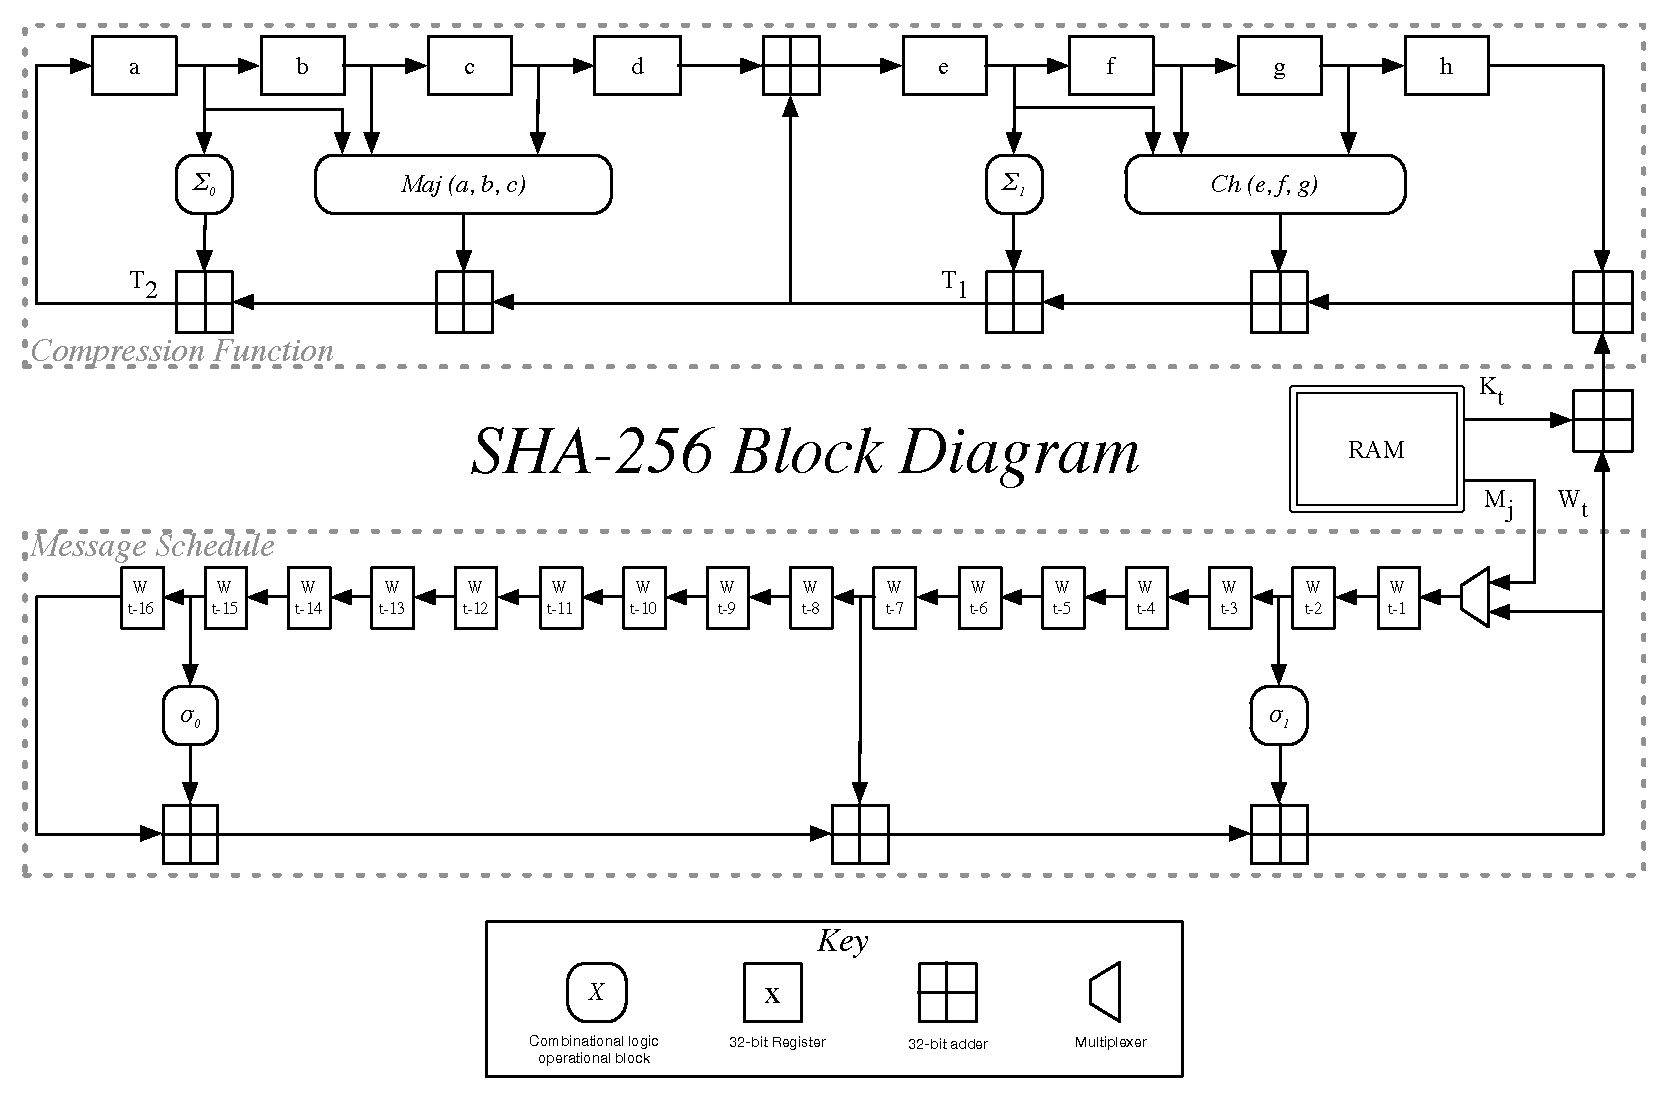
\includegraphics[angle=270, scale=0.7]{images/sha256}
  \caption{SHA-256 Block Diagram}
\end{figure}

\subsection{Implementation}

The internal implementation of a hash function can take many forms, however in
our case it must be through the use of linear feedback shift registers (LFSR)
throughout the design.

\section{True Random Number Generation on FPGA}
In Electronics a hardware clock is created from a harmonic oscillator such as a
quartz crystal whose output flips high to low and back at a regular interval.
The basics of the implementation of a random number generator to be used by the
fuzzy extractor is by sampling the output state of one hardware clock at times
controlled by another. We can utilise the clock drift as a source of randomness.
The two clocks are required to originate from two independent clock crystals
(one cannot be the Phased Locked Loop result of the other). Since a clocks
crystals are not perfectly precise in their oscillation due to thermal noise
effects ageing and variances in supply current and voltage it can be seen to be
unknown at a given time whether two independent clocks are in phase or not. 

If the frequency of one clock is very much higher than the other (1000s of
times), it can be seen as a type of digitised noise source in respect to the
readings that will be obtained at the sampling frequency imposed by the slower
clock.
However this implies that the bit rate of the output of the random number
generator will have to be very much lower than the fastest clock.
For the purposes of the Generation procedure in a Fuzzy extractor that is used
only once in a factory setting this issue may well not be a problem.
In reference to the implementation used the two random number generators used
need only to generate a few hundred bits of random data for each
Challenge//Response Pair.
Given that each generation procedure also required many clock cycles of activity
for BCH encoding and SHA-256 Hashing it would be possible to generate random
data of required length in the time it takes to complete a response.
However this random data is required at the start of the generation process,
therefore it would be expedient to generate the randomness required for the
first Fuzzy Extractor Generation Process during the devices initialisation
routines and store the result in a buffer. Then on subsequent generation
procedures, after the buffer contents has been accessed the random data
generation process can function in parallel, filling the buffer with new
randomness.

\section{Modified Ethernet Authentication Protocol Design}
% Chapter 4

\chapter{Results} % Chapter title

\label{ch:results} % For referencing the chapter elsewhere, use \autoref{ch:results}

%TC:ignore
%Results chapter should be approximately 2,000 Words in total.
%PUF section should be approximately 450 words long.
%Fuzzy Extractor section, it should be approximately 450 words long.
%Cryptographic Hashing section, it should be about 450 words long.
%Networking section, again, it should be 450 words in length.
%Summing up section, it should be 200 words long.
%TC:endignore
%-------------------------------------------------------------------------------

\section{SRAM-PUF}

In testing on various boards the extracted memory was found to exhibit large
differences in output given the same challenge, hence it c
ould informally be seen that there is a large \emph{inter-distance}.
Contrastingly, very little change was ever detected on any one single board
given multiple identical challenges, hence, informally, it would seem that
there is a small \emph{intra-distance}. The purpose of this project is
not to explore the performance of the IS61LV25616 \gls{sram} chip, so this was
not systematically tested, but it is reassuring to know that the chip had the
desired performance characteristics.

While the design was simulated in Mentor Graphic's Modelsim application using a testbench
during initial development, once
minimal functionality was achieved outside simulation the testbench was no longer
used. After further development of the system the testbench code no longer matches
with the implementation and so was deprecated and the earlier waveforms produced
are not included in this dissertation as they are no longer relevant.

The SRAM-PUF was extensively tested simply by connecting the serial cable to a
PC running a common serial terminal emulator. It was found to function well when
data was manually typed by a user, producing the correct 4 digits of hexadecimal
output (the memory contents of an \gls{sram} address) each time 4 corresponding hexadecimal digits
were entered (the memory address of \gls{sram} to select for output).

Timing issues were found to occur when data was sent automatically, either through
\matlab serial functions or through a line-oriented terminal mode. These were
mostly corrected, but issues still occurred when using different setups, lack of time
meant that these issues were never completely eliminated. The SignalTap application
was used to try and detect the source of the issues, but a lack of understanding
of its functionality meant that triggering never occurred correctly and the
investigation proved unfortunately fruitless. It is certain that more work is
required to bring this component up to the sought level of functionality, but
its ability to function manually was sufficient to complete the objectives of the
project.

\section{Fuzzy Extractor}

The results from the fuzzy extractor show that it functions correctly. Below is
a printout from a \matlab which demonstrates the fuzzy extractor running
eleven times. The first run (w) is the generator process providing the original
response (R) and the helper data (s and x). The next seven runs (wa05 - wa15)
are simulated reproduction runs wherein 5, 8, 9, 10 11, 12 and 15 errors are
introduced into the raw response. The last three (wr1 - wr3) simulate the
reproduction runs on non-authentic devices with different randomly generated
raw responses. Next the corresponding responses are given (R00-R15 \& RR1-RR3)
and the simulation concludes with the validation checking which shows that
up to ten errors can be mitigated. It also shows that when a raw response has a
hamming distance from the original greater than 10 the given digest response of
the fuzzy extractor has a hamming distance close to 50\%, i.e. the avalanche
effect of the cryptographic hash in the privacy amplification procedure is
effective in securing the response and preventing replay attacks:

\begin{verbatim}
w = D9DA7BEA1A31D8ABE2A27B4E855C5C5C
wa05 = D9DA6BEA1B31D8A3E2A27B4E857C5E5C
wa08 = D1D27BEA3A21D8ABE2A27B4E955D545E
wa09 = F9CA7BE21A71D8ABE2C27B4E855CDDDC
wa10 = DBEA7BCA1E21F8ABE2B27B4CA55C5C5C
wa11 = D0DA7BA81CB0D8ABE2E23B6E855C5C5C
wa12 = D1DA7BEA1A35DCBBE6B37B4AA15DDC5C
wa15 = D8DBFBEA5AB580ABE2B27B2E815C4C5E
wr1 = 7B86B5F833E9BF6A0EE6538261C5A7AE
wr2 = DD4DC9E1AAD2BB30051F0F6F2E1CB7F9
wr3 = BBD3AE3E9D8B3CE8867A027F0979F8F6

R = 5204AD19BDFA759B36D1CEF842B924C15A977F112E246CC4A5336E149058BDE6
s = 35B5595F99E4A446741CAFEE3F1C08C4
x = 37982001400E20B7A67AB050F073F429

R00 = 5204AD19BDFA759B36D1CEF842B924C15A977F112E246CC4A5336E149058BDE6
R05 = 5204AD19BDFA759B36D1CEF842B924C15A977F112E246CC4A5336E149058BDE6
R08 = 5204AD19BDFA759B36D1CEF842B924C15A977F112E246CC4A5336E149058BDE6
R09 = 5204AD19BDFA759B36D1CEF842B924C15A977F112E246CC4A5336E149058BDE6
R10 = 5204AD19BDFA759B36D1CEF842B924C15A977F112E246CC4A5336E149058BDE6
R11 = CB3B16EFADAB739429A5381A5F9C21E112D23487E933B0A7B6FCA4BDF4809B99
R12 = B01F5CFF14677D560D1CEBD5C876A458BA761B563622CD4C1413690454E8464F
R15 = 5225B4E08066191C29395423B0DCDA8F4B4C4DFB73CD254B1F57CAE5DD455E13
RR1 = 23DA1F0810BD6D6D73C1C61E659267F2132DF43BB729D1702A53944F754E941A
RR2 = DF0BC75A7A5D346B4E67FDD1A4CC67C0807E4ABFFD3F90A5BFDD70689B623B5D
RR3 = 43737B59470BFBA2056FD47B239536389EDAFF3B3AAA2FDBD63D8472269FA7D1

The R00 device passed verification
The R05 device passed verification
The R08 device passed verification
The R09 device passed verification
The R10 device passed verification
The R11 device failed verification, distance: 49.2%
The R12 device failed verification, distance: 44.1%
The R15 device failed verification, distance: 53.1%
The RR1 device failed verification, distance: 48.8%
The RR2 device failed verification, distance: 51.6%
The RR3 device failed verification, distance: 48.0%
\end{verbatim}

Next the ability to alter attributes of the fuzzy extractor is shown. The test
is the same, but this time the SRAM-PUF data width is halved to 64 bits and the
message length is correspondingly reduced to 30 bits. Thus only 6 bits can be
corrected. The output shown the fuzzy extractor performing accordingly:

\begin{verbatim}
w = 673E9620164BD71E
wa04 = 633E9660164BF71F
wa05 = 673A12201249D71E
wa06 = 672A8660364BD79E
wa07 = 6736DEA0024BD31E
wr1 = 410BCBA3D7C877AE
wr2 = 9B05581D6F8CEC6C
wr3 = F3BB6A432F7D979F

R = 3DAD18154B7010A439AA68448151F61E74A727229DB50D8576AC59EF2F353C81
s = 3C7F8142BE595539
x = 390F18C57D17BB8E

R00 = 3DAD18154B7010A439AA68448151F61E74A727229DB50D8576AC59EF2F353C81
R04 = 3DAD18154B7010A439AA68448151F61E74A727229DB50D8576AC59EF2F353C81
R05 = 3DAD18154B7010A439AA68448151F61E74A727229DB50D8576AC59EF2F353C81
R06 = 3DAD18154B7010A439AA68448151F61E74A727229DB50D8576AC59EF2F353C81
R07 = 741373A3B67B00242E02F0EE90D07A47C08DAB741086D39F7C0D46DF8CF37C71
RR1 = 0F1069EB2913962B55B410EA144BDC594AC97BA8A33CA94EA789FA539348A0BD
RR2 = 5A28A8EB40D64B96730CB9A45D26B0019EFAC0ECD0A09ABF4A994BD7349AEBB2
RR3 = 39B7AC78B67FEBA7C20273E24F178DB9B68985B16B22D621914B1D524F54CD60

The R00 device passed verification
The R04 device passed verification
The R05 device passed verification
The R06 device passed verification
The R07 device failed verification, distance: 43.8%
The RR1 device failed verification, distance: 52.3%
The RR2 device failed verification, distance: 53.1%
The RR3 device failed verification, distance: 53.9%
\end{verbatim}

\section{SHA-256}

The sha-256 implementation was tested to ensure it conformed with the standard
specification given in \cite{fips2001180} exactly. It was tested against the
worked example included in an official description document\cite{shsnist} and
implementations available on the web and iPhone apps. It was shown to follow
the specification exactly, as long as the message fits into one block.

The output generated from \matlab when running the implementation of SHA-256
against the hexadecimal encoding of the \gls{ascii} text `abc':

\begin{verbatim}
>> sha256('616263')
ans = BA7816BF8F01CFEA414140DE5DAE2223B00361A396177A9CB410FF61F20015AD
\end{verbatim}

This can be seen to be the same result as that given on page 11 of \cite{shsnist}.

\section{Ethernet Authentication}

Code to simulate the generation and extraction of data from Ethernet packets
with EAP-PUF protocol bodies were developed (see \autoref{app:eappuf}). The
resulting hexadecimal packets were constructed as follows:

\begin{description}
\item[EAPoL Start Packet (From Supplicant)] \hfill \\
\inlinecode{0180C200000300005E005301888E02010000} + 4 Byte CRC
\item[EAP Identity Request Packet (From Authenticator)] \hfill \\
\inlinecode{00005E00530100005E0053FF888E020000060155000601B0} + 4 Byte CRC
\item[EAP Identity Response Packet (From Supplicant)] \hfill \\
\inlinecode{00005E0053FF00005E005301888E0200000B0255000B0100005E005301} + 4 Byte CRC
\item[EAP EAP-PUF Request Packet (From Authenticator)] \hfill \\
\inlinecode{00005E00530100005E0053FF888E0200003501550035B0} + Challenge(16 Bytes)
                                               + Helper Data(32 Bytes)
                                               + 4 Byte CRC
\item[EAP EAP-PUF Response Packet (From Supplicant)] \hfill \\
\inlinecode{00005E0053FF00005E005301888E0200002502550025B0} + Response(32 Bytes)
                                               + 4 Byte CRC
\item[EAP Success Packet (From Authenticator)] \hfill \\
\inlinecode{00005E00530100005E0053FF888E0200000403550004} + 4 Byte CRC
\item[EAPoL Logoff Packet (From Supplicant)] \hfill \\
\inlinecode{0180C200000300005E005301888E02020000} + 4 Byte CRC
\end{description}

These Ethernet packet stubs have been checked and verified to correctly follow
the specification proposed.

\subsection{CRC}

The \gls{crc} algorithm is used to generate the \gls{fcs} appended to every
Ethernet packet. Below is the output of running the \matlab implementation
developed for this project against the EAPoL Start Packet as generated above:

\begin{verbatim}
>> crc('0180C200000300005E005301888E02010000')
ans = F7D19377
\end{verbatim}

This can be seen to be the same as the specification by checking using the online
\gls{fcs} generator at \inlinecode{http://www.lammertbies.nl/comm/info/crc-calculation.html}.

\section{Overall System Results}

The overall system was tested through a demonstration as shown in \autoref{fig:demo}.
While not all parts of the EAP-PUF protocol were simulated and there are still
issues with the \gls{uart} implementation in communicating effectively with \matlab,
in general terms the system can be said to be functional in a prototype form.

There is much that could be done to improve and develop the implementation, but
it shows in broad terms that the design proposed works, which was the intention
of the project.

\begin{figure}
  \centering
  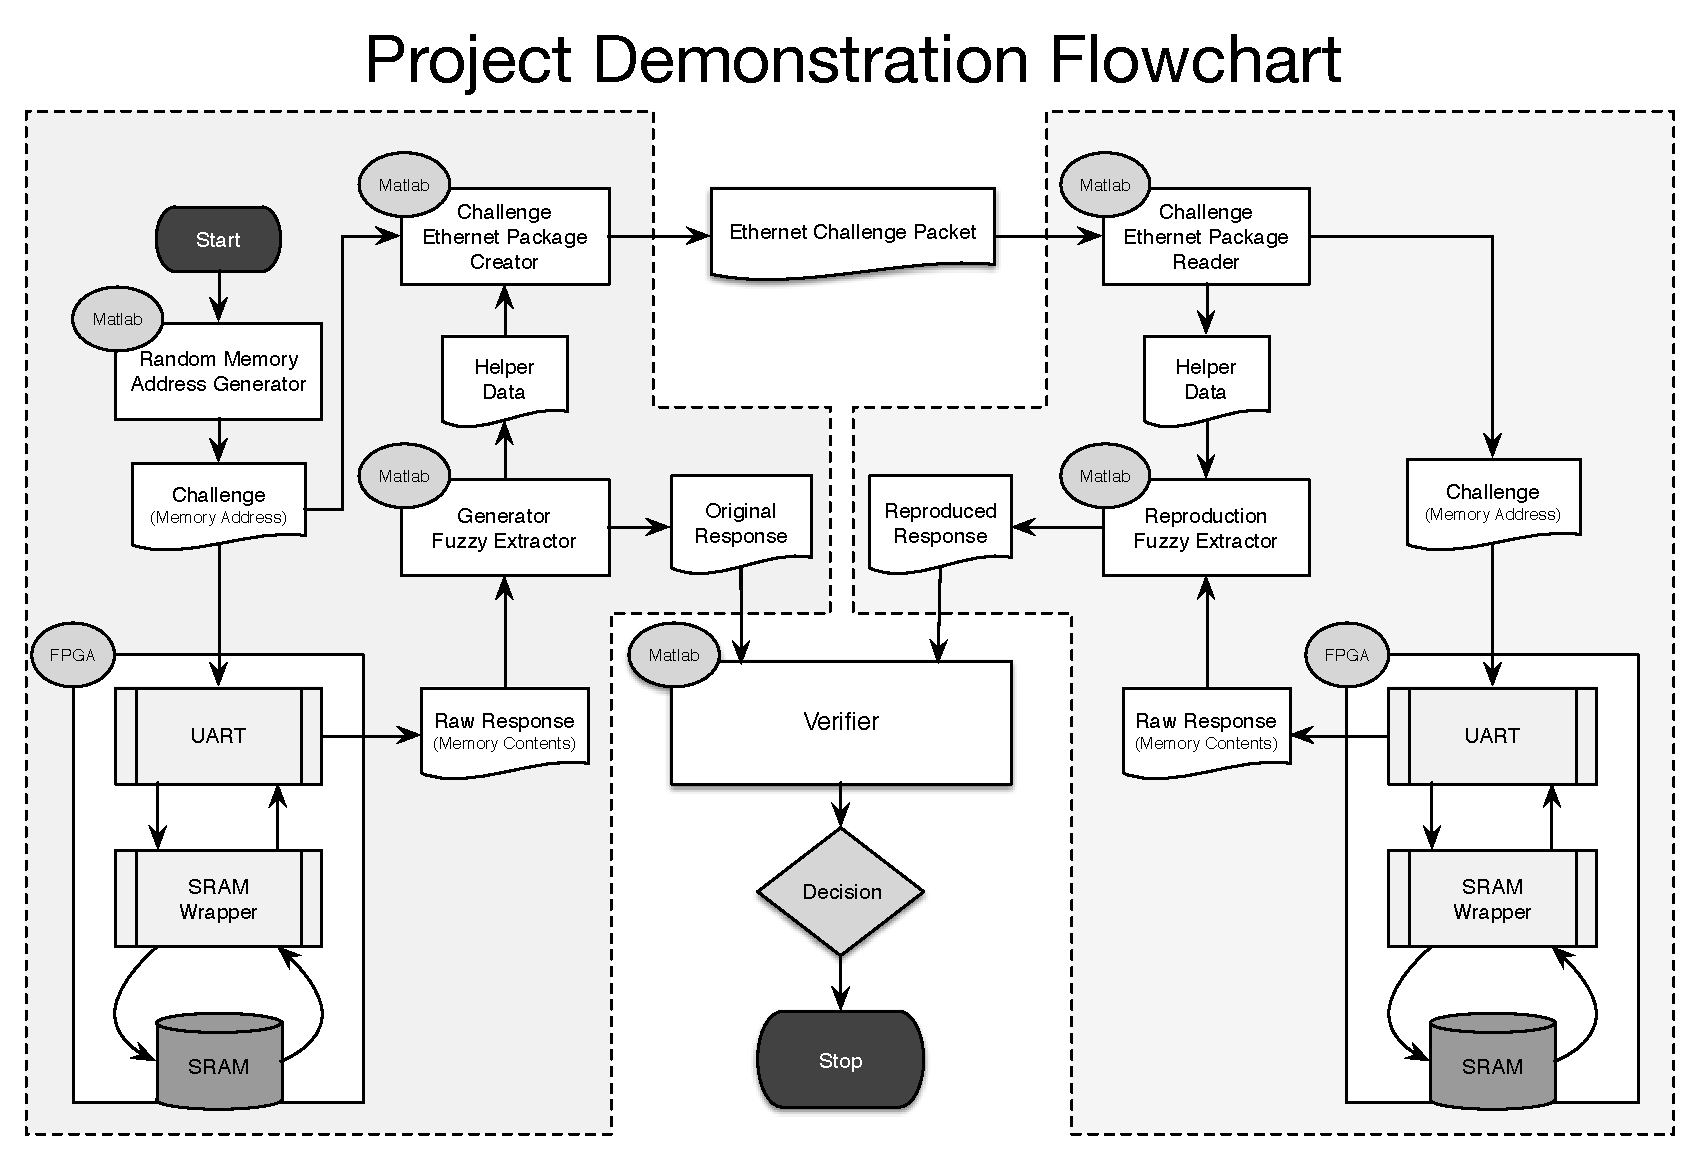
\includegraphics[angle=270, scale=0.8]{images/flowchart}
  \caption{Full system testing demonstration flowchart}
  \label{fig:demo}
\end{figure}

% Chapter 5

\chapter{Conclusion} % Chapter title

\label{ch:conclusion} % For referencing the chapter elsewhere, use \autoref{ch:conclusionn} 

%TC:ignore
This is the conclusion chapter, it should be approximately 750 Words
%TC:endignore
%-------------------------------------------------------------------------------

% Chapter 6

\renewcommand{\bibname}{References}
\bibliographystyle{IEEEtran}
\bibliography{dissertation}


References generated using $\mathrm{B{\scriptstyle{IB}} \! T\!_{\displaystyle E} \! X}$
% Appendix A

%-------------------------------------------------------------------------------
\appendix

\chapter{Appendix}

\section{Fuzzy Extractor Matlab Code}

\lstinputlisting[style=Matlab-editor]{../practical/matlab/fuzzy/fuzzytest.m}

\newpage

\section{SHA-256 Matlab Implementation}

\lstinputlisting[style=Matlab-editor]{../practical/matlab/sha256/sha256.m}
\lstinputlisting[style=Matlab-editor]{../practical/matlab/sha256/padmessage.m}
\lstinputlisting[style=Matlab-editor]{../practical/matlab/sha256/hexadd.m}
\lstinputlisting[style=Matlab-editor]{../practical/matlab/sha256/t1.m}
\lstinputlisting[style=Matlab-editor]{../practical/matlab/sha256/t2.m}
\lstinputlisting[style=Matlab-editor]{../practical/matlab/sha256/Maj.m}
\lstinputlisting[style=Matlab-editor]{../practical/matlab/sha256/Ch.m}
\lstinputlisting[style=Matlab-editor]{../practical/matlab/sha256/BigSigma0.m}
\lstinputlisting[style=Matlab-editor]{../practical/matlab/sha256/BigSigma1.m}
\lstinputlisting[style=Matlab-editor]{../practical/matlab/sha256/LittleSigma0.m}
\lstinputlisting[style=Matlab-editor]{../practical/matlab/sha256/LittleSigma1.m}


\section{Appendix III}

Third Appendix, probably some source code...

\section{Appendix IV}

Fourth Appendix, probably some source code...

\section{Appendix V}

Fifth Appendix, probably some source code...

\end{document}
